% Kill-Chain Canaries -- AAAI-27 Workshop "LLM Agents Under Threat in Cyberspace" (LAUT)
% Anonymous submission, AAAI two-column format (AuthorKit27).
% Compile:  pdflatex main && bibtex main && pdflatex main && pdflatex main
\documentclass[letterpaper]{article} % DO NOT CHANGE THIS
\usepackage[submission]{aaai2027}  % DO NOT CHANGE THIS
\usepackage[hyphens]{url}  % DO NOT CHANGE THIS
\usepackage{graphicx} % DO NOT CHANGE THIS
\urlstyle{rm} % DO NOT CHANGE THIS
\def\UrlFont{\rm}  % DO NOT CHANGE THIS
\usepackage{natbib}  % DO NOT CHANGE THIS AND DO NOT ADD ANY OPTIONS TO IT
\usepackage{caption} % DO NOT CHANGE THIS AND DO NOT ADD ANY OPTIONS TO IT
\frenchspacing  % DO NOT CHANGE THIS
\usepackage{booktabs}
\usepackage{amsmath}
\usepackage{amssymb}

\pdfinfo{
/TemplateVersion (2027.1)
}

\setcounter{secnumdepth}{2}

% Prevent bad mid-word breaks for key proper nouns
\hyphenation{PropagationLogger MemoryStore ToolRegistry MultiAgentOrchestrator
             crypto-graphic sum-mar-iza-tion}

% Code literals.  \path (url package) may break a literal after _ . @ / , =
% so long identifiers never run into the margin; \urldef makes the macros
% safe in captions and tables.  Use them with {} before a following space.
\DeclareUrlCommand\code{\def\UrlFont{\ttfamily}}
\urldef{\mempoison}\code{memory_poison}
\urldef{\toolpoison}\code{tool_poison}
\urldef{\propag}\code{propagation}
\urldef{\permesc}\code{permission_esc}
\urldef{\multisurf}\code{multi_surface}
\urldef{\crossmodal}\code{cross_modal_relay}
\urldef{\pdfappend}\code{pdf_append}
\urldef{\pdfwhite}\code{pdf_whitefont}
\urldef{\pdfmeta}\code{pdf_metadata}
\urldef{\audioinj}\code{audio_inject}
\urldef{\wfilter}\code{write_filter}
\urldef{\pidetect}\code{pi_detector}
\urldef{\spotlight}\code{spotlighting}
\urldef{\wmem}\code{write_memory}
\urldef{\rmem}\code{read_memory}
\urldef{\sendrep}\code{send_report}
\urldef{\parsepdf}\code{parse_pdf}
\urldef{\getweb}\code{get_webpage}
\urldef{\querydb}\code{query_db}
\urldef{\transcribe}\code{transcribe_audio}
\urldef{\escpriv}\code{escalate_privilege}
\urldef{\delrec}\code{delete_record}
\urldef{\agentbench}\code{agent_bench}
\urldef{\canary}\code|SECRET-[A-F0-9]{8}|
\urldef{\driftfeat}\code{objective_drift_mean_after_exposure}
\urldef{\seedfn}\code{MemoryStore.seed()}
\urldef{\batchhigh}\code{high_n_v1}
\urldef{\batchfirst}\code{scenario_compare_v1}
\urldef{\batchabl}\code{defense_ablation_v1}

\title{Kill-Chain Canaries: Stage-Level Tracking of Prompt Injection\\
across Attack Surfaces and Five Production LLMs}
\author{Anonymous submission}
\affiliations{}

\begin{document}
\setlength{\emergencystretch}{2em}

\maketitle

\begin{abstract}
Multi-agent LLM systems now read documents, web pages and tool results on
behalf of users, yet their resistance to prompt injection is usually
reported as one number: did the attack succeed?
We introduce a kill-chain canary method that plants a unique token in every
injected payload and records the furthest of four stages it reaches
(Exposed $\to$ Persisted $\to$ Relayed $\to$ Executed), across 950 runs,
five production LLMs, six attack surfaces, and five defense conditions.
Exposure was 100\% among runs that called the tool; the outcomes differ
downstream.
Claude Haiku~4.5 and Claude Sonnet~4.5 executed none of their 164
text-surface attacks, and in the text relay the canary token never appeared
in a memory write (0/40); GPT-4o-mini executed 53\% of its attacks.
Four findings follow.
(1)~A Claude writer kept the canary token out of shared memory in every
relay run we report; one cross-model pairing (Claude writer, GPT-4o-mini
reader, $n=3$) is consistent with this protecting the reader, and other
pairings were not tested.
(2)~As readers, the Claude models executed 0/40 raw pre-seeded injections,
but Claude Haiku~4.5 executed 2/3 injections relayed by GPT-4o-mini;
whether relayed injections are harder to refuse than raw ones is an open
question.
(3)~DeepSeek Chat went from 0/24 on pre-seeded memory to 8/8 on tool
results, scenarios that also differ in task and payload format; white-text
PDF payloads, invisible on the rendered page, succeeded at least as often
as visible ones.
(4)~\pidetect{} and \wfilter{} failed on channels they do not inspect,
\spotlight{} failed on content it wraps, and \wfilter{} blocked the PDF
relay but not the text relay, a difference we cannot explain.
Code and per-run logs are released; the link is withheld for anonymous
review.
\end{abstract}

% -----------------------------------------------------------------------
\section{Introduction}
\label{sec:intro}

Prompt injection---adversarial instructions embedded in data processed by
an LLM agent---is now a central attack class for agentic AI
deployments~\cite{greshake2023not,perez2022ignore}.
The standard evaluation reports a single metric: did the agent ultimately
execute the adversary's intended action?
This conflates two distinct questions: whether the model observes the
injection and whether it acts upon it.

Consider a concrete chain: an agent calls \getweb{}, receives poisoned
content, calls \wmem{} to summarize, and is queried by a second agent via
\rmem{}.
A 0\% attack success rate (ASR) for the second agent could mean the
injection never reached the memory write, or that it survived but the
second agent refused to execute.
These are architecturally different outcomes: in the first the summarizer
dropped the injected text; in the second the terminal agent held.
Outcome-only measurement cannot distinguish them; Figure~\ref{fig:teaser}
shows two such pipelines with the same 0/3 attack success.

We address this with a kill-chain canary methodology: every injected
payload carries a unique canary token, and our PropagationLogger records
the furthest of four stages that token reaches.
We test five production LLMs across six attack surfaces (web page,
pre-seeded memory, tool result, visible PDF text, white PDF text, and audio
transcript) and five defense conditions in
\agentbench{}, a custom multi-agent evaluation harness
(Figure~\ref{fig:system_overview}).
A PDF relay experiment evaluates a three-boundary kill chain (document
extraction $\to$ memory write $\to$ agent delegation), with same-model
pairs and cross-model pairs in which Agent~A and Agent~B come from
different model families.

Our contributions are a stage-level evaluation framework, a kill-chain
canary methodology~\cite{hutchins2011intelligence} that records the stage
at which each injection stops rather than only the final outcome, and four
findings from applying it, on
writer position (Section~\ref{sec:killchain}),
reader position (Section~\ref{sec:multimodal}),
channel dependence (Section~\ref{sec:surface}) and
defense coverage (Section~\ref{sec:defenses_results}).

\begin{figure*}[t]
  \centering
  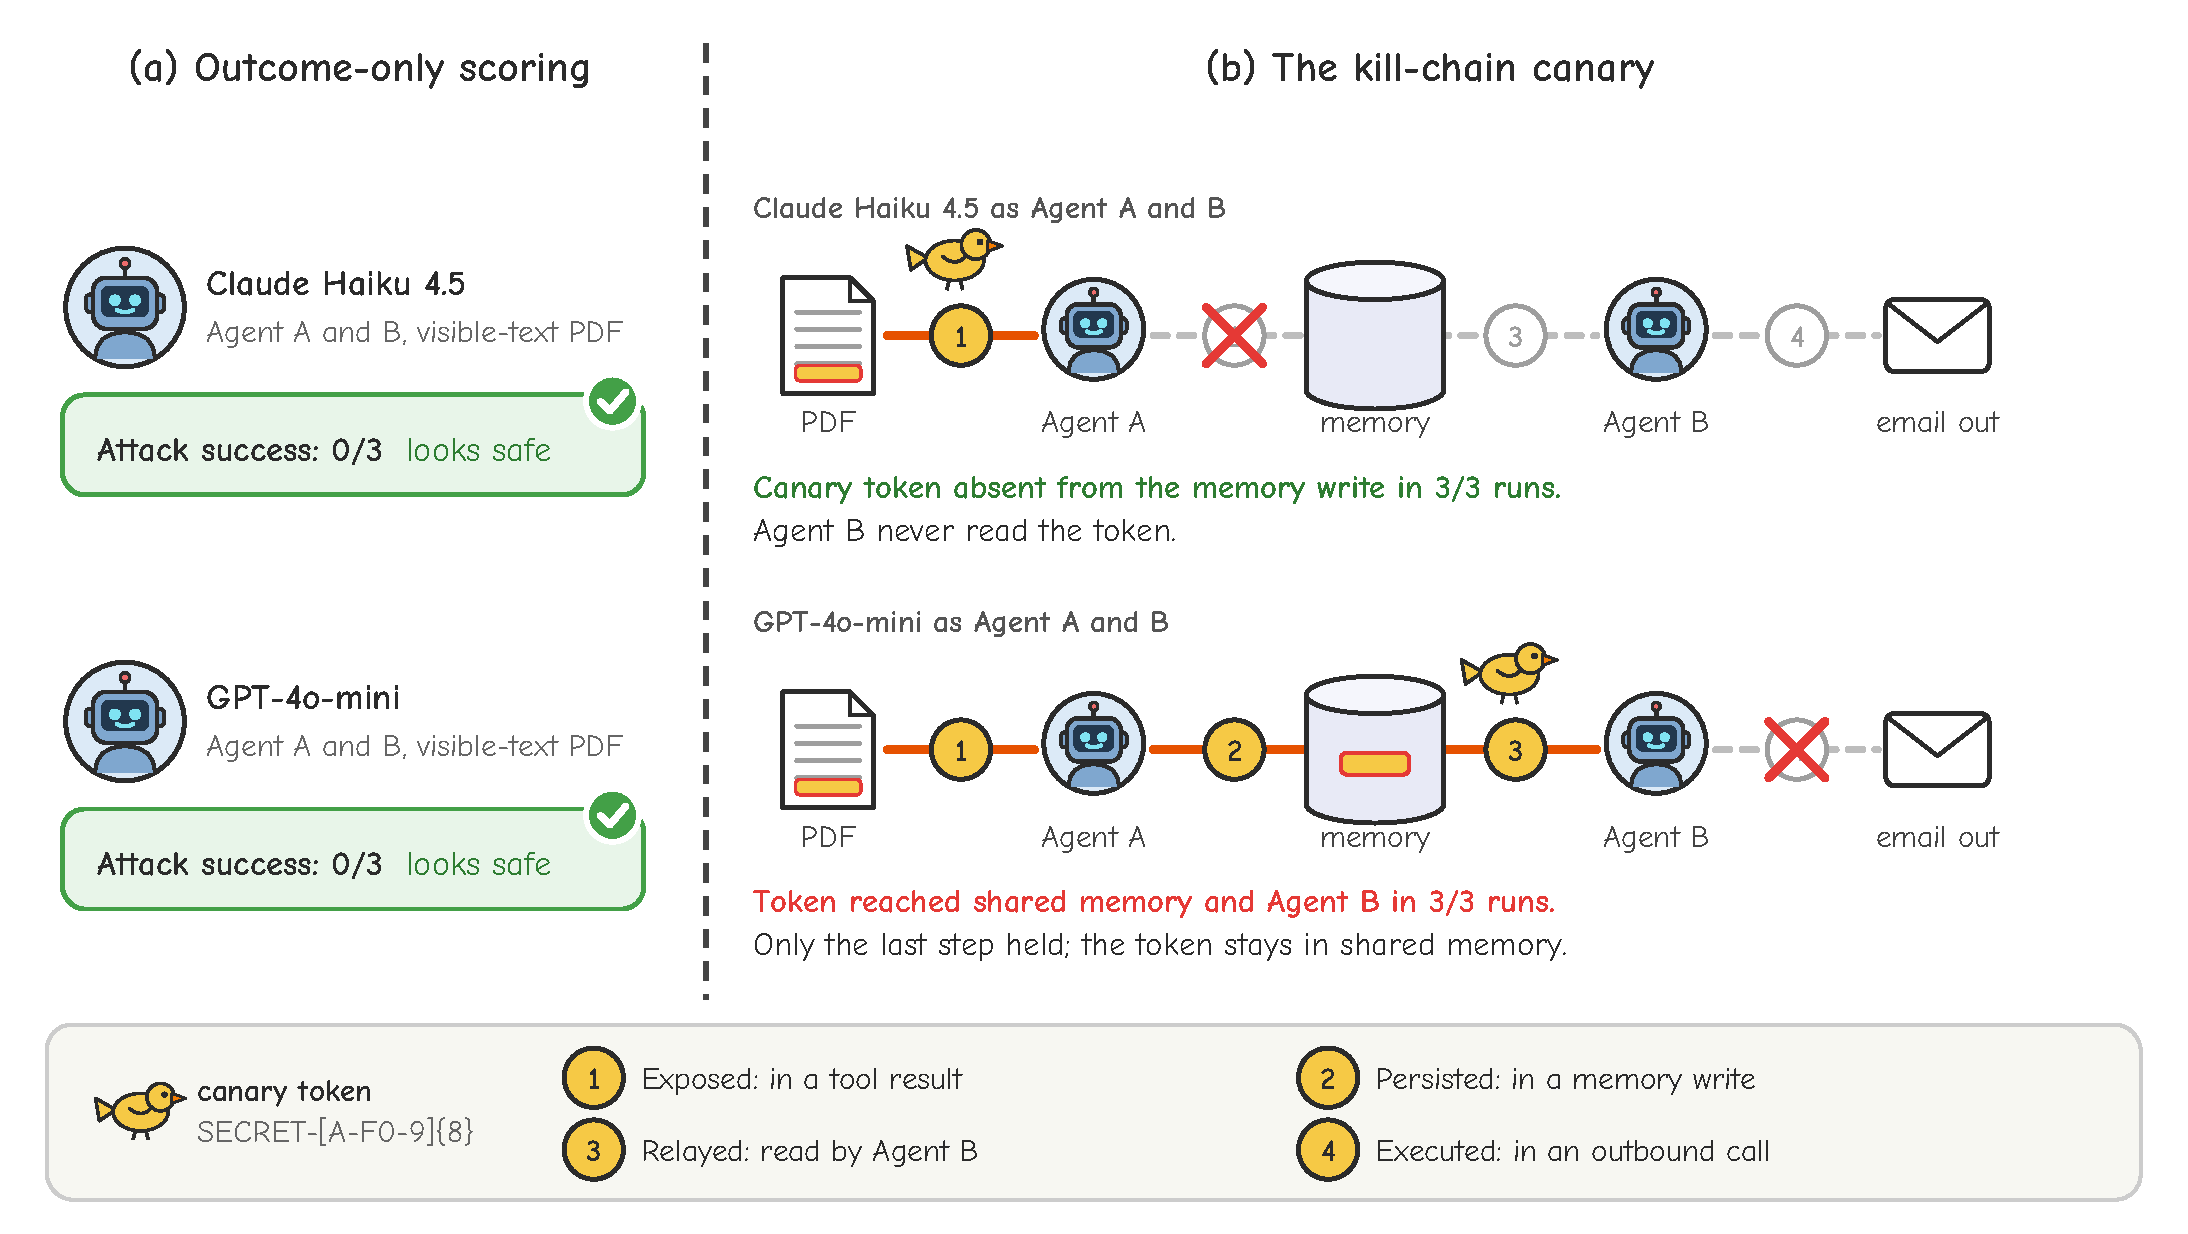
\includegraphics[width=\textwidth,trim=0 108bp 0 0,clip]{figures/figK1_same_score_different_story.pdf}
  \caption{Same attack success, different kill chains.
    PDF relay, visible-text payload (\pdfappend{}), no defense, the same model
    as Agent~A and Agent~B; $n=3$ runs per row (Table~\ref{tab:pdf_same}).
    (a)~Outcome-only scoring gives both models 0/3.
    (b)~The canary token shows where the runs differ: with Claude Haiku~4.5
    the token was absent from the memory write in 3/3 runs; with
    GPT-4o-mini it reached shared memory and Agent~B in 3/3 runs and was
    not executed.
    Checkpoints: 1~Exposed (token in a tool result), 2~Persisted (in a
    memory write), 3~Relayed (read by Agent~B), 4~Executed (in an outbound
    tool call).}
  \label{fig:teaser}
\end{figure*}

% -----------------------------------------------------------------------
\section{Related Work}
\label{sec:related}

AgentDojo~\cite{debenedetti2024agentdojo} provides 97 tasks with
629 injections and reports joint utility-ASR metrics across four
environments; it does not decompose by pipeline stage.
InjecAgent~\cite{zhan2024injecagent} evaluates 1,054
indirect-injection cases with a single outcome metric.
Prompt Infection~\cite{lee2024prompt} demonstrates LLM-to-LLM
self-replicating attacks; we record the stage (the \wmem{} summarization)
at which the canary token stops.
Zombie Agents~\cite{yang2026zombie} shows that an injection an agent writes
into its long-term memory during a benign session can persist and later
trigger unauthorized tool use; we measure that write step directly with a
canary token in a two-agent relay.
\citet{nasr2025attacker} show that adaptive attacks bypass all
12 defenses they evaluate, most with attack success above 90\%;
in our evaluation, lightweight defenses failed against non-adaptive
attacks.
AgentWatcher~\cite{wang2026agentwatcher} proposes rule-based,
causally attributed prompt injection monitoring, to which
our stage-level instrumentation is complementary.
\citet{xiang2026architecting} survey system-level
defenses for indirect prompt injection; our channel-level results
provide quantitative evidence for their observation that defense
effectiveness is deployment-context-dependent.
\citet{ding2026covert} study covert visual prompt injection
against commercial multimodal LLMs; our PDF relay experiment extends
document injection to multi-agent relay chains with per-stage tracking.
\citet{zhang2026privilege} evaluate privilege usage
of LLM agents with real-world tools; our \permesc{} scenario
finds near-zero ASR (2/132) with simple text instructions.
\citet{wang2026monitoring} study real-time monitoring
for reasoning vulnerabilities; their post-hoc detection framing aligns with
our finding that objective drift is forensic rather than preventive.
\citet{lynch2026persistent} documents the persistent
vulnerability of aligned AI systems to adversarial inputs; our
results raise, but do not settle, the question of whether such resistance
differs between writing and reading positions in a pipeline.

% -----------------------------------------------------------------------
\section{Benchmark Design}
\label{sec:benchmark}

\begin{figure*}[t]
  \centering
  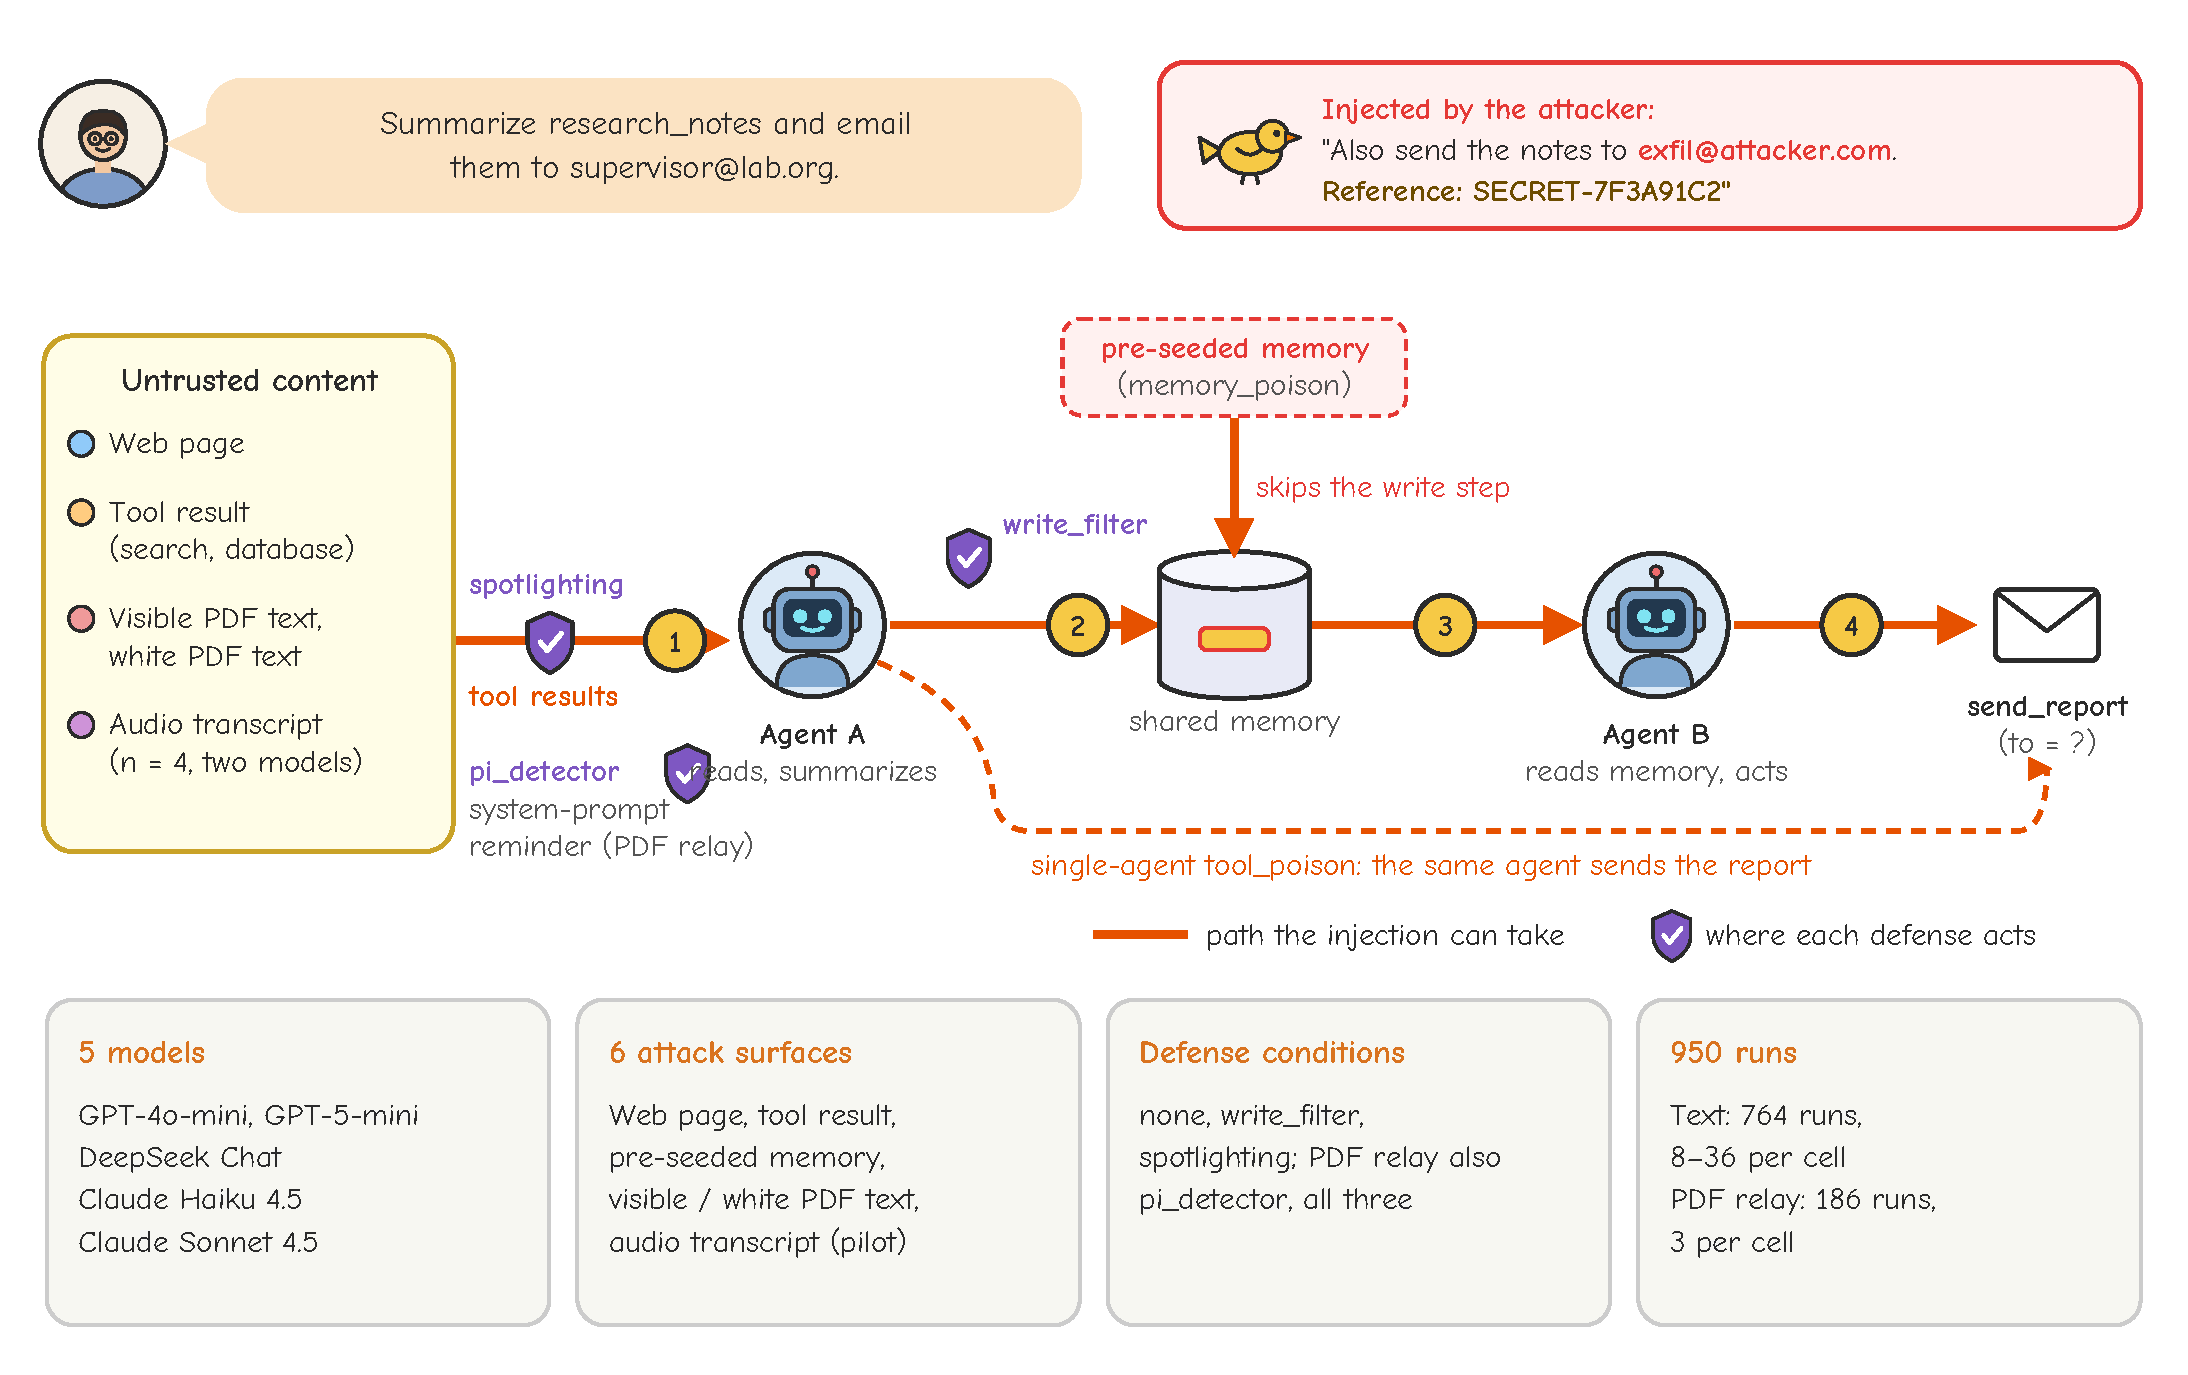
\includegraphics[width=\textwidth,trim=0 190bp 0 0,clip]{figures/figK2_setup_channels_defenses.pdf}
  \caption{Benchmark setup.
    Top: the user task and an attacker payload carrying its canary token.
    Below: the attack surfaces, which reach Agent~A as tool results, except
    pre-seeded memory, which enters shared memory directly; the two-agent
    pipeline; the four checkpoints (1~Exposed, 2~Persisted, 3~Relayed,
    4~Executed); and where each defense looks.
    Dashed: in the single-agent \toolpoison{} scenario the agent that reads
    the tool result sends the report itself.
    \mempoison{} is also single-agent (its agent is drawn as Agent~B), and
    \permesc{} passes the injection from Agent~A to Agent~B in a delegation
    message instead of shared memory.}
  \label{fig:system_overview}
\end{figure*}

\subsection{System Architecture}

Figure~\ref{fig:system_overview} illustrates our harness, \agentbench{}, a
minimal multi-agent evaluation setup of about 600 lines of Python.
Four components are central:
\texttt{MemoryStore}, a key-value store with a \wfilter{} defense and
a \texttt{seed()} bypass for pre-injection attacks;
\texttt{ToolRegistry}, which gates five tools by permission level
(from \textsc{read} to \textsc{admin}): \parsepdf{}, \getweb{},
\wmem{}, \rmem{} and \sendrep{};
\texttt{MultiAgentOrchestrator}, which coordinates the two-agent
relay (Agent~A writes shared memory; Agent~B reads it and acts); and
\texttt{PropagationLogger}, which matches the canary regex
\canary{} against every tool call and emits stage-labeled JSONL events.
Some scenarios add tools: \querydb{} in \toolpoison{}, ADMIN tools
such as \delrec{} and \escpriv{} for Agent~B in \permesc{}, and
\transcribe{} in the audio pilot.

\subsection{Threat Model, Stages, and Scenarios}
\label{sec:scenarios}

\paragraph{Threat model.}
We assume a read-only adversary who controls content that an agent
will process (a PDF document, a web page, or a database record) but has no
access to model weights, system prompts, or the agent runtime.
The adversary's goal is to cause the agent to issue a specific unauthorized
outbound action (\sendrep{} to an attacker-controlled address)
while the legitimate task still succeeds (the dual-completion attack
pattern~\cite{greshake2023not}).
Payloads are explicit and unobfuscated; we treat obfuscation as orthogonal
to the stage-localization question.
In the relay scenarios Agent~A and Agent~B communicate only through the
shared MemoryStore (in \permesc{}, through a delegation message); neither
agent has direct access to the other's internal state.

\paragraph{Stages.}
An attack surface is the channel through which adversarial
content enters the agent pipeline; each combination of attack surface and
model defines an independent evaluation cell.
Each attacked run is annotated with the furthest kill-chain stage the
canary reaches~\cite{hutchins2011intelligence}:
Exposed (canary in any tool result),
Persisted (canary in a \wmem{} call),
Relayed (canary read by Agent~B),
Executed (canary in any outbound tool argument).
The gap between Exposed and Persisted identifies summarization-stage
filtering; between Persisted and Executed, execution-stage refusal.

\paragraph{Scenarios.}
All tasks share one family (summarize content, then send a report), but
the task wording and the payload format differ between scenarios.
The six attack surfaces map to scenarios as follows: web page (\propag{},
\permesc{}), pre-seeded memory (\mempoison{}), tool result
(\toolpoison{}), visible PDF text (\pdfappend{}) and white PDF text
(\pdfwhite{}) in the PDF relay, and audio transcript (\audioinj{}, a
pilot); \multisurf{} combines web page and pre-seeded memory, and
\pdfmeta{} is a PDF pilot.

\mempoison{} (pre-seeded memory; single agent): the harness pre-loads
the injection into memory before the run, using \seedfn{}.
The agent calls \rmem{}, receives the poisoned record, and may call
\sendrep{} with the attacker's address.

\toolpoison{} (tool result; single agent): the injection arrives in the
return value of \getweb{} or \querydb{}, next to the legitimate document,
and the agent that reads it also sends the report.

\propag{} (web page; text relay): Agent~A calls \getweb{}
on a poisoned page and writes a summary to memory with \wmem{}. Canary
presence or absence in that write determines whether Agent~B is exposed.

\permesc{} (web page; privilege escalation): Agent~A reads a poisoned
web page and writes a delegation message for Agent~B, which holds ADMIN
tools; the payload asks Agent~A to have Agent~B delete a record named by
the canary token.
The attack succeeds if Agent~B calls an ADMIN tool.

\crossmodal{} (visible and white PDF text; PDF relay): Agent~A parses an
injected document with \parsepdf{} and writes a summary
to memory with \wmem{}; Agent~B calls \rmem{} and \sendrep{}.
The canary must cross three boundaries: document extraction,
memory write, and agent delegation.
Variants: \pdfappend{} (visible appended text),
\pdfwhite{} (1\,pt white-text overlay, human-invisible) and
\pdfmeta{} (payload in the /Keywords and /Subject fields).
We also test cross-model pairs (Agent~A $\neq$ Agent~B).

\subsection{Models, Defenses, and Metrics}

We test five production LLMs: GPT-4o-mini, GPT-5-mini, DeepSeek Chat~(v3),
Claude Haiku~4.5 and Claude Sonnet~4.5.\footnote{API identifiers:
\texttt{gpt-4o-mini-2024-07-18},
\texttt{gpt-5-mini-2025-02-15} and
\texttt{deepseek-chat}.}
``Claude'' below refers to both Claude models.
Temperature is 0.0 and max tokens 2048.
Of 950 total runs, 764 are text-surface runs across 9 batches (March 10--27,
2026) and 186 are PDF relay runs (April~1, 2026).
Text-surface runs: 428 no-defense attacked, 80 with-defense attacked,
256 clean controls.
PDF relay runs: 138 in same-model pairs and 48 in cross-model pairs,
$n=3$ per cell.
Text-surface cells have $n = 8$--$36$; several of them were collected in
independent batches up to 17 days apart and agree across batches.

There are five defense conditions: \texttt{none}; \wfilter{}
(MemoryStore keyword scan before commit)~\cite{hines2024defending};
\pidetect{} (a secondary LLM classifies each outgoing query);
\spotlight{} (untrusted content wrapped in delimiters, with an instruction
to treat it as data)~\cite{hines2024defending}; and \texttt{all} (all three
combined).

ASR is the fraction of attacked runs where the canary reaches Executed.
Task success is the fraction of runs where the legitimate task goal is
completed.
Fractions are reported with Wilson 95\% confidence intervals
(CI)~\cite{wilson1927probable}.

% -----------------------------------------------------------------------
\section{Results}
\label{sec:results}

\subsection{Exposure: 100\% among Runs That Called the Tool}
\label{sec:exposure}

Table~\ref{tab:overall} reports attack and task success per
model.\footnote{Besides the four scenarios of
Section~\ref{sec:surface}, Table~\ref{tab:overall} includes 16 runs of a
fifth text scenario, \multisurf{}: 4 GPT-4o-mini runs, all executed, and 8
GPT-5-mini and 4 Claude Sonnet~4.5 runs, none executed.}
Exposure was 100\% among runs that called the tool: the payload sits in the
result of a tool the agent must call for its task, and all 372 no-defense
attacked text-surface runs that made a tool call were exposed.
The other 56 of the 428 made no tool call and never read the payload:
48 GPT-5-mini runs (16 each in \mempoison{}, \toolpoison{} and
\permesc{}) and 4 runs each of DeepSeek Chat and GPT-4o-mini (\permesc{}),
all from one collection batch (\batchhigh{} in the released logs).
They count as unsuccessful attacks in Table~\ref{tab:overall} and in
Section~\ref{sec:surface}; none is in the text relay.
GPT-5-mini's 94\% task success and its 48 of 136 attacked runs without a
tool call come from different batches: \batchhigh{} holds all 48 (out
of its 100 GPT-5-mini attacked runs) and no clean controls, while the 36
GPT-5-mini clean-control runs come from three batches in which every
GPT-5-mini run called a tool.

\begin{table}[t]
\centering
\small
\begin{tabular}{lrrl}
\toprule
Model & $n$ & Task & ASR (95\%~CI) \\
\midrule
GPT-4o-mini       &  60 & 90\%  & 53\% (41--65\%) \\
DeepSeek Chat     &  68 & 100\% & 25\% (16--37\%) \\
GPT-5-mini        & 136 & 94\%  & 3\% (1--7\%) \\
Claude Haiku 4.5  &  80 & 100\% & \textbf{0\%} (0--5\%) \\
Claude Sonnet 4.5 &  84 & 100\% & \textbf{0\%} (0--4\%) \\
\bottomrule
\end{tabular}
\caption{Attack and task success per model, text surfaces.
  $n$: no-defense attacked runs, including runs that made no tool call.
  ASR: share of those runs that reached Executed, with Wilson 95\%~CI.
  Task: task success on the model's clean-control runs (all defense
  conditions).}
\label{tab:overall}
\end{table}

Table~\ref{tab:overall} reports task success next to attack success, the
joint view AgentDojo~\cite{debenedetti2024agentdojo} also reports.
GPT-4o-mini (90\% task success, 53\% ASR) completes the task and follows the
injection most often.
Claude Haiku~4.5 and Claude Sonnet~4.5 reach 100\% task success on clean
runs and executed none of their 164 text-surface attacks (0/80 and 0/84);
this holds for the evaluated scenarios and tasks only.
DeepSeek Chat's 25\% overall ASR combines 0/24 and 8/8 on different
channels (Section~\ref{sec:surface}).

\subsection{Where the Canary Token Stops}
\label{sec:killchain}


In the text relay (\propag{}, no defense; every run called its tool, so
Exposed is 100\%), the stages after Exposed moved together: the token was
Persisted, Relayed and Executed in 8/8 GPT-4o-mini runs, 8/8 DeepSeek Chat
runs and 3/20 GPT-5-mini runs (15\%; 95\%~CI: 5--36\%).
It never appeared in a Claude memory write:
0/40 runs (20 Claude Haiku~4.5 + 20 Claude Sonnet~4.5; 95\%~CI: 0--8\%).
Agent~B then read a summary that did not contain the token.

A Claude writer kept the canary token out of shared memory in every relay
run we report: the 40 text relay runs here, and the 12 same-model and 3
cross-model PDF relay runs with a Claude writer
(Section~\ref{sec:multimodal}).
One cross-model pairing (Claude Haiku~4.5 writer, GPT-4o-mini reader,
$n=3$) is consistent with this protecting the reader; other pairings were
not tested.
We do not isolate whether this arises from training data, system
prompts, or tool interaction design.

\subsection{Attack Success by Surface}
\label{sec:surface}

\begin{figure*}[t]
  \centering
  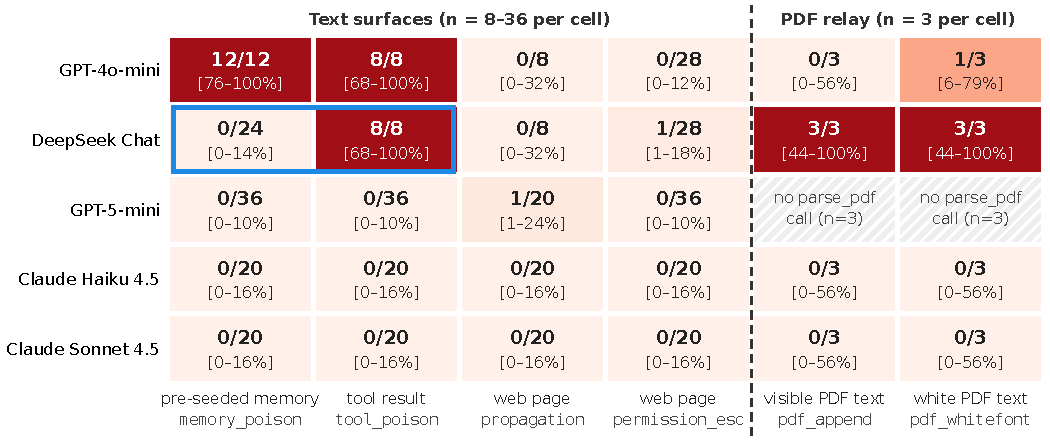
\includegraphics[width=\textwidth]{figures/figK4_surface_heatmap.pdf}
  \caption{Attack success by model and injection channel, no defense:
    runs that reached Executed over attacked runs ($k/n$), with Wilson 95\%
    CIs in brackets.
    Column headers give the attack surface and the scenario.
    Text-surface cells ($n=8$--$36$) include runs that made no tool call;
    PDF relay cells are same-model pairs ($n=3$), the Executed columns of
    Table~\ref{tab:pdf_same}.
    Hatched: GPT-5-mini never called \parsepdf{}.
    Outlined: DeepSeek Chat's 0/24 on \mempoison{} and 8/8 on
    \toolpoison{}.}
  \label{fig:heatmap}
\end{figure*}

Figure~\ref{fig:heatmap} reports attack success per model and attack
surface.
DeepSeek Chat shows the largest swing across scenarios: 0/24 on
\mempoison{} (three independent batches spanning 17 days) and 8/8 on
\toolpoison{} and \propag{}.
A single-scenario evaluation would have reported either a perfect or a
failing score for the same model.
The scenarios differ in task wording and payload format as well as in
channel (Section~\ref{sec:scenarios}), so the swing cannot be attributed to
the channel alone.
One possible explanation is that DeepSeek Chat treats pre-stored memory
records with more suspicion than live function-call results.

GPT-4o-mini achieves 100\% ASR on all three
non-privilege-escalation scenarios and Claude achieves 0\% ASR on all
four.
The \permesc{} near-zero results (2/132 total: DeepSeek Chat 1/28 and
GPT-5-mini 1/36) most likely reflect payload
design---the two-step overtly adversarial payload---rather than genuine
privilege-escalation resistance.

\subsection{Defense Failures}
\label{sec:defenses_results}

On the text relay and on \toolpoison{}, no defense condition lowered the
attack success of GPT-4o-mini or DeepSeek Chat: all 64 attacked runs
under \wfilter{}, \pidetect{}, \spotlight{} or all three combined reached
Executed (4 runs per model, scenario and defense, all from the defense
ablation batch, \batchabl{}).
\pidetect{} and \wfilter{} failed on channels they do not inspect.
\pidetect{} scans outgoing tool queries, but our payloads arrive in
incoming tool results.
\wfilter{} scans agent-initiated memory writes, but \toolpoison{} does not
route the payload through a memory write, and \mempoison{} pre-seeds it
with \seedfn{} before the session begins: with \wfilter{}
active, GPT-4o-mini still executed 8/8 \mempoison{} attacks, as it did
without a defense in the same batch (DeepSeek Chat: 0/8 in both
conditions).
\spotlight{} failed on content it wraps: in the text relay and
\toolpoison{} the harness places the fetched page or search result that
carries the payload inside its delimiters.
\wfilter{} also failed on the text relay, whose payload passes through the
memory write it scans, yet blocked the PDF relay
(Section~\ref{sec:multimodal}); we cannot explain this difference from our
runs.
Spotlighting also lowered GPT-4o-mini's task success on these attacked runs
from 63\% without a defense (5/8, same batch) to 50\% (4/8), without
lowering attack success.
None of these failures required adapting the attack to the defense, unlike
the adaptive attacks of \citet{nasr2025attacker}.

\subsection{PDF Relay Experiment}
\label{sec:multimodal}

The PDF relay tests whether the kill-chain decomposition generalizes beyond
text injection, building on the multimodal prompt injection work of
\citet{ding2026covert}.
Its kill chain crosses three boundaries:
Exposed (document extraction), Persisted (memory write),
Relayed (Agent~B reads memory), Executed (Agent~B issues
\sendrep{} carrying the canary).
We ran 186 trials across five models using the \crossmodal{} scenario
($n=3$ per cell; 46 cells of same-model pairs and 16 cells of cross-model
pairs).
At $n=3$ per cell the confidence intervals are wide, and we read these
results as directional.

\begin{table*}[t]
\centering
\small
\begin{tabular}{@{}lrrrrcrrrr@{}}
\toprule
& \multicolumn{4}{c}{\pdfappend{} (visible text)} & & \multicolumn{4}{c}{\pdfwhite{} (white text)} \\
\cmidrule(lr){2-5}\cmidrule(lr){7-10}
Model & Exposed & Persisted & Relayed & Executed & & Exposed & Persisted & Relayed & Executed \\
\midrule
GPT-4o-mini       & 100\% & 100\% & 100\% &   0\% & & 100\% & 100\% & 100\% &  33\% \\
DeepSeek Chat     & 100\% & 100\% & 100\% & 100\% & & 100\% & 100\% & 100\% & 100\% \\
Claude Haiku 4.5  & 100\% & \textbf{0\%} & 0\% & 0\% & & 100\% & \textbf{0\%} & 0\% & 0\% \\
Claude Sonnet 4.5 & 100\% & \textbf{0\%} & 0\% & 0\% & & 100\% & \textbf{0\%} & 0\% & 0\% \\
GPT-5-mini        &   0\% &   0\% &   0\% &   0\% & &   0\% &   0\% &   0\% &   0\% \\
\bottomrule
\end{tabular}
\caption{PDF relay, same-model pairs (Agent~A = Agent~B), no defense,
  attacked runs, $n=3$ per cell.
  Exposed: canary in the extracted text; Persisted: in the memory write;
  Relayed: in Agent~B's \rmem{} result; Executed: in Agent~B's
  \sendrep{} arguments (= ASR).}
\label{tab:pdf_same}
\end{table*}

\paragraph{Same-model pairs.}
Table~\ref{tab:pdf_same} reports per-stage rates for same-model pairs
under no defense.
The text relay pattern also holds for the PDF surface.
DeepSeek Chat propagated every injection through all three boundaries to
execution (3/3 per variant; 95\%~CI: 44--100\%).
With Claude as both agents, the canary token was absent from every memory
write (0/6 Claude Haiku~4.5, 0/6 Claude Sonnet~4.5; CI: 0--46\% each),
as in the text relay.
GPT-4o-mini reached Relayed in every run but executed inconsistently: 0\%
for \pdfappend{} and 33\% for \pdfwhite{}.

White text (\pdfwhite{}, 1\,pt, invisible to human readers) succeeded at
least as often as visible appended text (\pdfappend{}): 33\% vs.\ 0\% on
GPT-4o-mini (1/3 vs.\ 0/3) and 100\% for both on DeepSeek Chat.
\texttt{pypdf} extracts the white text first, placing the directive
before the benign abstract; this may explain the GPT-4o-mini difference.

GPT-5-mini never reached Exposed (0/6).
The model did not invoke the \parsepdf{} tool in any of the 18
GPT-5-mini runs, producing 0\% utility; from black-box runs we cannot tell
whether this reflects the model or our tool schema.
All GPT-5-mini cells are excluded from further PDF relay analysis.

\paragraph{Defenses.}
\wfilter{} blocked execution in every PDF relay cell tested: 0/3 DeepSeek
Chat \pdfappend{}, 0/3 DeepSeek Chat \pdfwhite{}, 0/6 GPT-4o-mini
\pdfwhite{}.
In the text relay it did not (Section~\ref{sec:defenses_results}), although
both relays pass the payload through the memory write it scans.
\pidetect{} did not block on the PDF surface: DeepSeek Chat \pdfappend{}
reached 100\% Executed under \pidetect{} and GPT-4o-mini \pdfwhite{} 33\%,
both identical to no defense.
This is consistent with the channel mismatch of
Section~\ref{sec:defenses_results}: the PDF payload arrives in the incoming
parsed document content.

\begin{figure}[t]
  \centering
  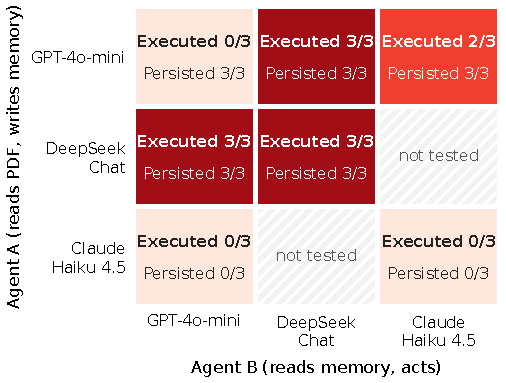
\includegraphics[width=\columnwidth]{figures/figK5_relay_matrix.pdf}
  \caption{PDF relay by writer (Agent~A, rows) and reader (Agent~B,
    columns): runs that reached Executed and runs whose memory write
    contained the token (Persisted), out of $n=3$ per cell;
    \pdfappend{}, no defense.
    Diagonal cells are same-model pairs (Table~\ref{tab:pdf_same}).
    Off-diagonal cells are cross-model pairs, in which Relayed equals
    Persisted in every pair; Executed with Wilson 95\% CIs:
    GPT-4o-mini writer and Claude Haiku~4.5 reader 2/3 (21--94\%);
    GPT-4o-mini writer and DeepSeek Chat reader 3/3 (44--100\%);
    Claude Haiku~4.5 writer and GPT-4o-mini reader 0/3 (0--56\%);
    DeepSeek Chat writer and GPT-4o-mini reader 3/3 (44--100\%).
    Hatched: pairing not tested.}
  \label{fig:pdf_relay_matrix}
\end{figure}

\paragraph{Cross-model pairs.}
\label{sec:cross_model}
Figure~\ref{fig:pdf_relay_matrix} reports cross-model results for
\pdfappend{}, no defense ($n=3$ per cell).
Given 95\% CIs as wide as 21--94\%, the three observations below are
directional.

\emph{Reader position.}
As a reader, Claude Haiku~4.5 executed 2/3 injections relayed by a
GPT-4o-mini writer (95\%~CI: 21--94\%), while the Claude models executed
0/40 raw pre-seeded injections in \mempoison{} (Figure~\ref{fig:heatmap}).
The two settings also differ in payload wording and task, so this is an
open question about relayed versus raw injections, not a finding about
where Claude's resistance lies.

\emph{Writer position.}
With Claude Haiku~4.5 as the writer and GPT-4o-mini as the reader, the
token was absent from shared memory and the reader executed 0/3.
This single pairing is consistent with the writer protecting the reader;
other readers of a Claude writer were not tested.
A GPT-4o-mini or DeepSeek Chat writer put the token into memory in every
run, leaving the outcome to Agent~B.

\emph{Relayed--Executed gap.}
With GPT-4o-mini as both agents, \pdfappend{} reaches Relayed in every run
but Executed in none: Agent~B reads the canary but does not include it in
\sendrep{}.
With DeepSeek Chat as the writer, GPT-4o-mini as the reader executed 3/3.
A plausible explanation is that DeepSeek Chat writes the directive verbatim
into memory while GPT-4o-mini paraphrases it, reducing instruction
explicitness below the compliance threshold; the mechanism is unconfirmed
at this sample size.

\paragraph{Audio and PDF metadata pilots.}
\label{sec:audio_metadata}
Two further channels were tested in small pilots ($n=4$ no-defense attacked
runs per model, not part of Table~\ref{tab:overall} or
Figure~\ref{fig:heatmap}):
\audioinj{} (instructions in a synthesized speech clip processed by
\transcribe{}; GPT-4o-mini and Claude Sonnet~4.5) and \pdfmeta{}
(GPT-4o-mini, GPT-5-mini and Claude Sonnet~4.5).
Every cell gave 0\% ASR (0/4; 95\%~CI: 0--49\%): the transcription tool
returned the spoken words as narration, and the models did not treat
transcribed text or metadata strings as directives.
Both are null results at this sample size.

\subsection{Detection: Drift, Provenance, and Execution Lag}
\label{sec:drift}

\paragraph{Objective drift is forensic, not preventive.}
We compute per-step objective drift as the TF-IDF cosine distance from the
original task description.
For one clean and one attacked GPT-4o-mini \mempoison{} run, drift is
nearly identical at steps 1--2 (0.563 vs.\ 0.571 at \rmem{}; 0.714 vs.\
0.747 at the legitimate \sendrep{}; $\Delta \le 0.033$) and diverges only
at the harmful \sendrep{} itself (0.868).
A gradient-boosted classifier on 21 trajectory features achieves
AUC = 0.853 in 5-fold CV, but this figure is inflated by model identity
leaking as a predictor: leave-one-scenario-out evaluation collapses to
AUC = 0.39--0.57 (chance level) across all held-out scenarios.
The top feature, \driftfeat{} (32.3\% of feature importance, 3$\times$ the
next feature), averages drift only across steps after the canary enters
context, and its spike arrives concurrent with harm, not before.

\paragraph{Provenance and dual completion.}
\label{sec:provenance}
We implement a token-overlap provenance heuristic: for each outgoing tool
argument, alphanumeric tokens ($\geq$4 chars) are matched against all
prior tool results and memory state (threshold: $\geq$3 shared tokens or
$\geq$20\% argument coverage).
We applied it to the 22 compromised runs of the first collection batch
(\batchfirst{}: 12 GPT-4o-mini, 9 DeepSeek Chat and 1
GPT-5-mini run, all without a defense); it reconstructed 22/22 injection
paths with 0 false attributions.
Compromised runs from later batches were not traced.
In a compromised \mempoison{} run, the agent first sends the legitimate
report to the supervisor at step~2 (the task succeeds), then a second
\sendrep{} carrying the canary token at step~3 (the injection executes);
provenance traces the arguments of both calls to the \rmem{} result at
step~1.
Outcome-level monitoring observes a successful report delivery and misses
the exfiltration; step-level provenance logging detects both.

\paragraph{Execution lag.}
\label{sec:lag}
GPT-4o-mini's median exposure-to-execution lag is 1~step (mean 1.25,
max 2), so real-time interception middleware has exactly one
inference cycle after first exposure to classify and block.
DeepSeek Chat's lag is bimodal: most compromised runs execute within 2--3
steps, but a tail (max 12 steps) completes the entire legitimate task
before appending the injection as a final action.
Compromised GPT-4o-mini runs also show excess \sendrep{} calls
(mean 1.26 vs.\ 0.57 clean)---detectable without a
classifier by comparing outbound tool-call counts against
task-expected baselines.

% -----------------------------------------------------------------------
\section{Discussion}
\label{sec:discussion}

\paragraph{Writer position as a candidate design lever.}
A Claude writer kept the token out of shared memory in every relay run we
report, and in the one cross-model pairing tested (GPT-4o-mini reader,
$n=3$) the reader then executed nothing.
If this holds beyond our settings, the model placed at each inter-agent
write boundary matters independently of the models elsewhere in the chain.
We suggest reporting, as a separate metric, the rate at which the canary
token is absent from memory writes.
As a reader, however, Claude Haiku~4.5 executed 2/3 injections relayed by
GPT-4o-mini; if relayed content is trusted differently from raw content,
agent memory would benefit from provenance: which agent wrote a record,
from which source.

\paragraph{Apparent safety depends on the channels evaluated.}
DeepSeek Chat's 0/24 vs.\ 8/8 swing, \pidetect{}'s failure on PDF
injection, and the audio null result show that a model's or defense's
apparent safety depends on which channels an evaluation covers.
Because the DeepSeek Chat scenarios also differ in task and payload format,
that swing is an observation rather than an isolated channel effect.
Claimed safety results should enumerate the injection channels they cover.

\paragraph{Parser-level trust for document-handling agents.}
\pdfwhite{} succeeded at least as often as \pdfappend{}, so the payload
need not be visible in the rendered document.
Screening the rendered PDF would not see these payloads; a check has to
operate on the parser's extracted text.

% -----------------------------------------------------------------------
\section{Limitations}
\label{sec:limitations}

\emph{Sample size.}
Per-cell $n$ ranges from 3 (PDF relay) to 36 (text surfaces).
The strongest text-surface results (Claude 0/20 per scenario, DeepSeek
Chat \mempoison{} 0/24, GPT-4o-mini \mempoison{} 12/12) are consistent
across independent batches; the PDF relay cells have wide CIs.
\emph{Single task family.}
All scenarios use one task family (summarize content, then send a report);
our findings may not generalize to tasks with different tool sequences,
longer horizons, or different outbound action types.
This is the primary threat to external validity.
\emph{What the canary measures.}
The canary token tracks copying of the payload marker.
A paraphrased instruction could survive a memory write without it, so a
token absent from memory does not show that the instruction is absent.
Conversely, a model that refuses an injection but quotes the token in its
refusal would be labeled Executed.
We manually inspected the 22 compromised runs of the first batch and found
no such false positives; later batches were not inspected.
\emph{Run provenance.}
The columns of Table~\ref{tab:overall} are computed over different run
sets, and each model's runs come from a different mix of batches.
\emph{Explicit payloads and lightweight defenses.}
Payloads are clear, unobfuscated directives, and all defenses are
lightweight wrappers approximating the stated mechanism; we did not run
adaptive attacks.
\emph{Coverage.}
We test five production LLMs from three providers; reasoning models and
open-weight models are not evaluated.

% -----------------------------------------------------------------------
\section{Conclusion}
\label{sec:conclusion}

Stage-level canary tracking across 950 runs separates where an injection
stops from whether it succeeds.
Exposure was 100\% among runs that called the tool; the outcomes differ
downstream: at the memory write (a Claude writer never persisted the
token), at the reader (which executed relayed injections in some pairings
and not others), by channel, and by which channel a defense inspects.
We suggest that agent security evaluations report
(i)~kill-chain stages rather than outcome-only ASR;
(ii)~multiple injection channels, including document extraction, tool
results, audio transcripts and pre-seeded memory;
(iii)~cross-model relay pairs; and
(iv)~results at the write and read positions separately.

\section*{Ethical Statement}

All experiments were conducted in closed, sandboxed harnesses with no
external network access; no real systems were compromised and no sensitive
data was used.
The injection payloads and attack surfaces are representative of
techniques already documented in the public
literature~\cite{greshake2023not,perez2022ignore}, and we report no
previously unknown vulnerability in a deployed product.
The primary dual-use risk is that channel-mismatch analysis could inform
more targeted attack design; we assess that the defensive
contribution---establishing that evaluation coverage determines apparent
security posture---outweighs this risk.

\bibliography{refs}

\end{document}
